\documentclass{article}
\usepackage{tikz}
\usepackage{natbib}
\title{MCMC problems}
\date{}
\usepackage{caption}
\captionsetup{font=footnotesize}
\usepackage[utf8]{inputenc}
\usepackage{amsmath}
\usepackage{graphics}
\usepackage{graphicx}
\newtheorem{problem}{Problem}[section]
\usepackage{bbm}
\usepackage{listings}
\usepackage{minted}
\author{Ben Lambert}

\begin{document}
\maketitle

\section{Ticked off}
Imagine you are investigating the occurrence of Lyme disease in the UK. This is a vector-borne disease caused by bacteria of species \textit{Borrelia} which is carried by ticks. (The ticks pick up the infection by blood-feeding on animals/humans that are infected with \textit{Borrelia}.) As such, you decide to estimate the prevalence of this bacteria in ticks you collect from the grasslands and woodlands around Oxford.

As previously, you decide to use sample sizes of 100 ticks, out of which you count the number of ticks testing positive for \textit{Borrelia}. You decide to use a binomial likelihood since you assume that the presence of \textit{Borrelia} in one tick is independent of that in other ticks. Also because you sample a relatively small area you assume that the presence of \textit{Borrelia} can be assumed to be identically-distributed across ticks. 

\begin{problem}
In a single sample you find that there are 6 ticks that test positive for \textit{Borrelia}. Assuming a Beta(1,1) prior analytically calculate the posterior distribution. (Hint: by analytically here I mean look up the result on Google/in the lecture notes.) Graph this distribution. 
\end{problem}

Since the Beta prior here is conjugate to the Binomial likelihood the posterior is also a Beta distribution. To transform a Beta prior into a posterior, we use the rule: $Beta(a,b)\rightarrow Beta(a+X,b+n-X)$, where $(a,b)$ are the prior parameters, $X$ is the number of ticks collected and $n$ is the sample size. Since we are using a Beta(1,1) prior here, the posterior is a Beta(7,95) distribution; which has a posterior mean of $\frac{7}{102}\approx 0.069$.

\begin{problem}
Generate 100 independent samples from this distribution using your software's inbuilt (pseudo-)random number generator. Graph this distribution. How does it compare to the pdf of the exact posterior? (Hint: in R the command is ``rbeta''; in Matlab it is ``betarnd``; in Mathematica it is ``RandomVariate[BetaDistribution...]''; in Python it is ``numpy.random.beta''.)
\end{problem}

After only 100 independent samples the estimated posterior is quite similar in shape to the actual distribution (figure \ref{fig:ticks_independentVersusActual}).

\begin{figure}[ht]
\centerline{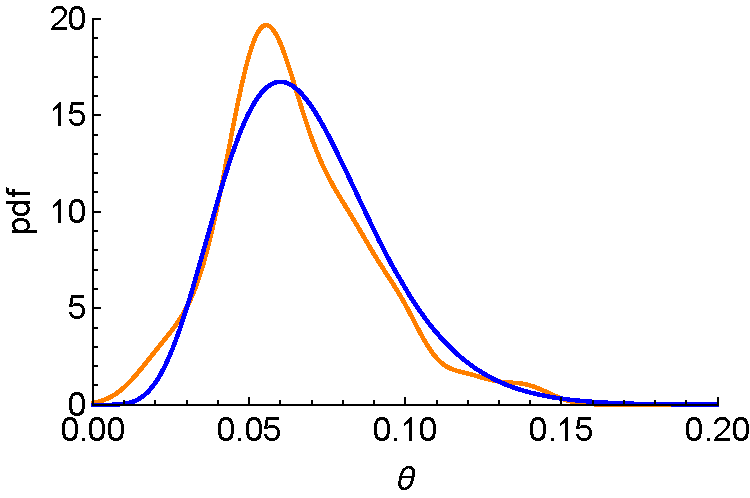
\includegraphics[width=0.8\textwidth]{../figures/prob3_ticks_independentSamples.pdf}}
\caption{A pdf of the posterior estimated from independent samples (orange) versus the exact posterior (blue).}\label{fig:ticks_independentVersusActual}
\end{figure}

\begin{problem}
Evaluate the effect of increasing the sample size for your independent sampler on the estimate of the mean of the distribution. (Hint: for each sample you are essentially comparing the sample mean with the true mean of the posterior.)
\end{problem}

The error in using independent sampling to estimate the mean of a distribution is given by the (Lindberg-Levy) central limit theorem:

\begin{equation}
(\bar{X}-\mathrm{E}[X]) \xrightarrow{d} N(0,\sigma)
\end{equation}

which means we can estimate the error for a large sample of size $n$ by:

\begin{equation}
(\bar{X} - \mathrm{E}[X]) \approx N(0,\frac{\sigma}{\sqrt{n}})
\end{equation}

This means that as the sample size increases the error in estimation decreases in accordance with $\sqrt{n}$ (figure \ref{fig:ticks_independentSampleSize}).

\begin{figure}[ht]
\centerline{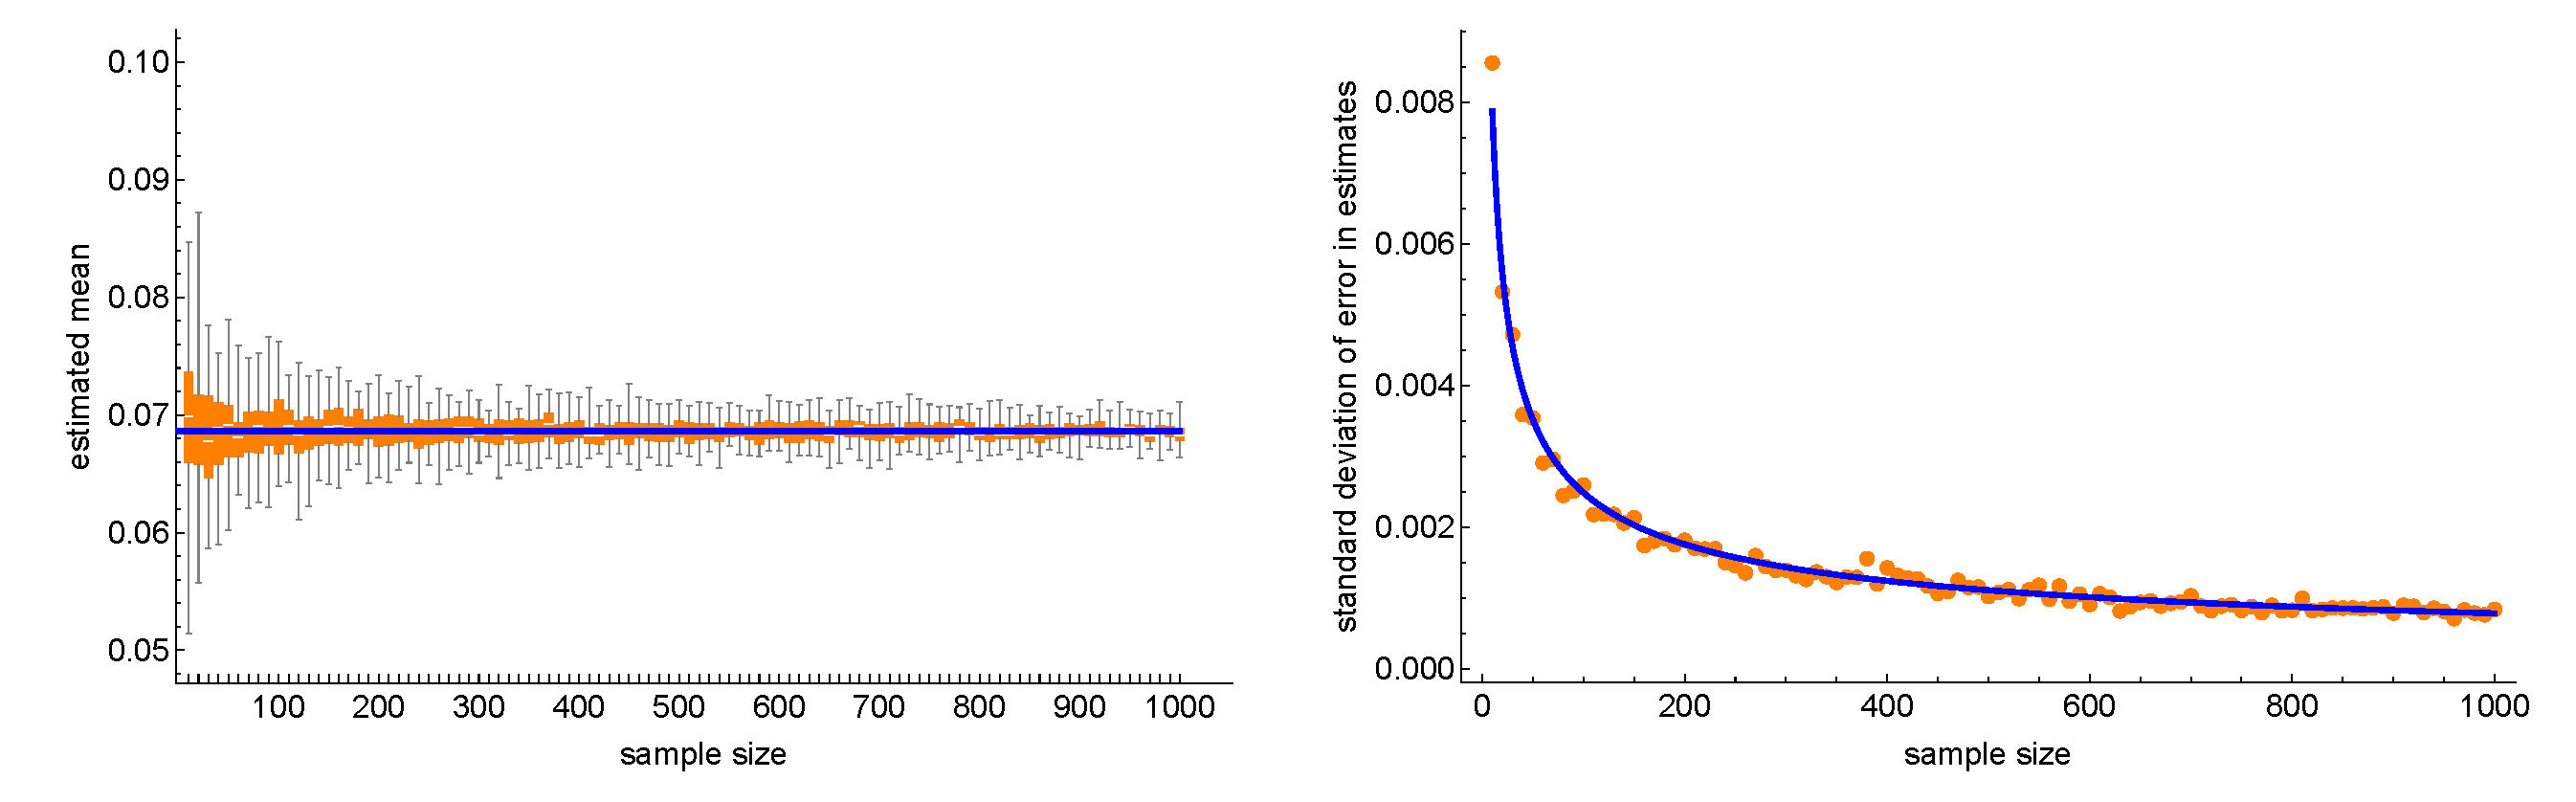
\includegraphics[width=1.5\textwidth]{../figures/prob3_ticksIndependentSampleSize.pdf}}
\caption{The estimated mean (left) and standard deviation in the error (right) using independent sampling to estimate the mean of the posterior for the ticks example.}\label{fig:ticks_independentSampleSize}
\end{figure}

\begin{problem}
Estimate the variance of the posterior using independent sampling for a sample size of 100. How does your sample estimate compare with the exact solution?
\end{problem}

To do this generate an independent sample of size 100, and calculate the sample variance (see figure  \ref{fig:ticks_independentVariance}.) Even after 100 samples we are able to estimate the posterior variance with quite reasonable resolution.

\begin{figure}[ht]
\centerline{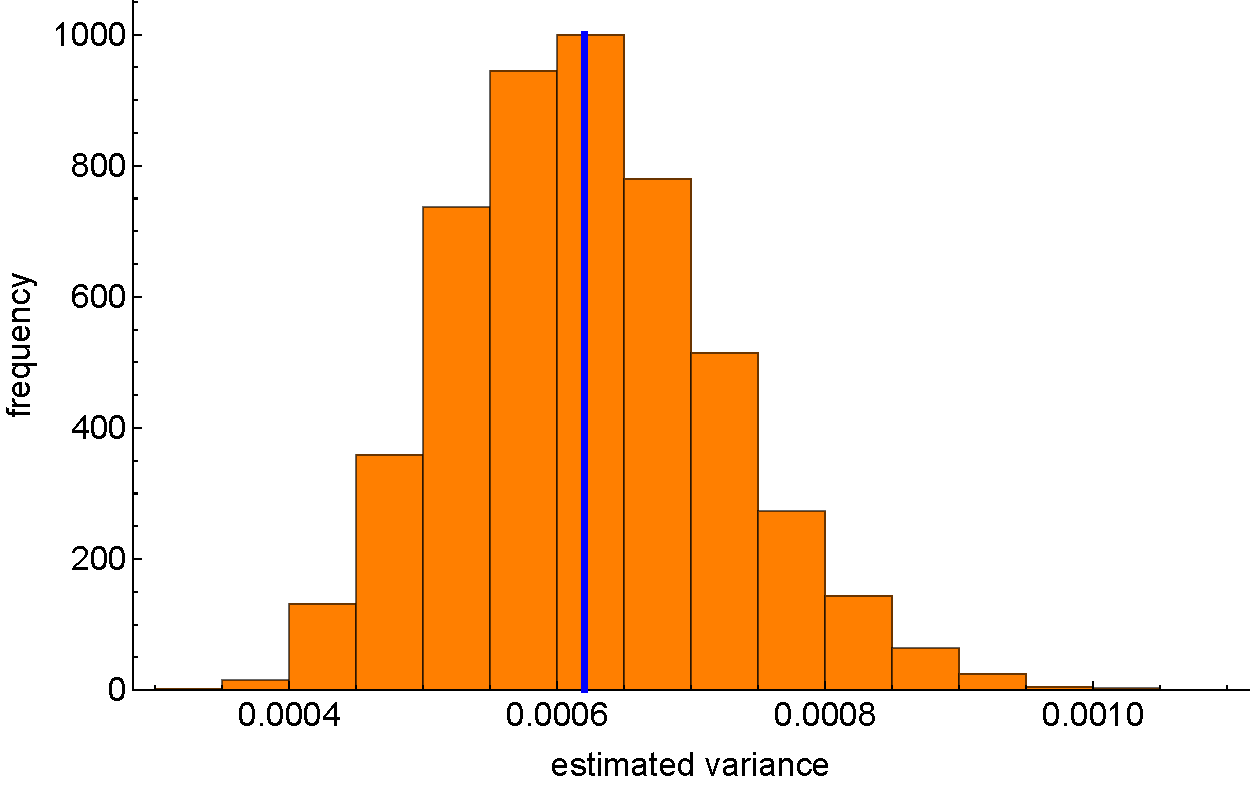
\includegraphics[width=1\textwidth]{../figures/prob3_ticksIndependentVariance.pdf}}
\caption{The estimated variance of the posterior for the ticks example versus the actual value (blue line) for an independent sample of size 100.}\label{fig:ticks_independentVariance}
\end{figure}

\begin{problem}
Create a proposal function for this problem that takes as input a current value of $\theta$, along with a step size, and outputs a proposed value. For a proposal distribution here we use a normal distribution centred on the current $\theta$ value with a standard deviation (step size) of 0.1. This means you will need to generate a random $\theta$ from a normal distribution using your statistical software's inbuilt random number generator. (Hint: the only slight modification you need to make here is to ensure that we don't get $\theta < 0$ or $\theta > 1$ is to use periodic boundary conditions. To do this we use modular arithmetic. In particular we set $\theta_{proposed} = mod(\theta_{proposed},1)$. The command for this in R is $x \%\% 1$; in Matlab the command is $mod(x,1)$; in Mathematica it is $Mod[x,1]$; in Python it is $x \% 1$.)
\end{problem}

\begin{problem}
Create the ``accept/reject'' function of Random Walk Metropolis that accepts as input $\theta_{current}$ and $\theta_{proposed}$ and outputs the next value of $\theta$. This is done based on a ratio:

\begin{equation}
r = \frac{p(X|\theta_{proposed}) \times p(\theta_{proposed})}{p(X|\theta_{current}) \times p(\theta_{current})}
\end{equation}

and a uniformly-distributed random number between 0 and 1, which we call $a$. If $r > a$ then we update our current value of $\theta_{current} \rightarrow \theta_{proposed}$; alternatively we remain at $\theta_{current}$. 
\end{problem}

\begin{problem}
Create a function that is a combined version of the previous two functions; so it takes as input a current value of $\theta_{current}$, generates a proposed $\theta_{proposed}$, and updates $\theta_{current}$ in accordance with the Metropolis accept/reject rule.
\end{problem}

\begin{problem}
Create a full-working Random Walk Metropolis sampler! (Hint: you will need to iterate the last function repeatedly. As such, you will need to decide on a starting position for $\theta$. I would recommend that you use a uniformly-distributed random number between 0 and 1.)
\end{problem}

\begin{problem}
For a sample size of 100 from your Metropolis sampler compare the sampling distribution to the exact posterior. How does the estimated posterior compare with that obtained via independent sampling using the same sample size?
\end{problem}

The MCMC sample distribution is not as crisp as the independent sample distribution (figure \ref{fig:ticks_independentMCMCIndependentExact}). This is because of the effects of dependence on the sampling efficiency. Intuitively, the information conveyed from each incremental sample is less than for the independent case. 

There is also a slight bias in the MCMC posterior towards the starting point of the algorithm. This is because sampler hasn't had sufficient time to converge to the posterior. This bias can be removed by using more samples from the posterior and discarding those samples during the ``warm-up'' period.

\begin{figure}[ht]
\centerline{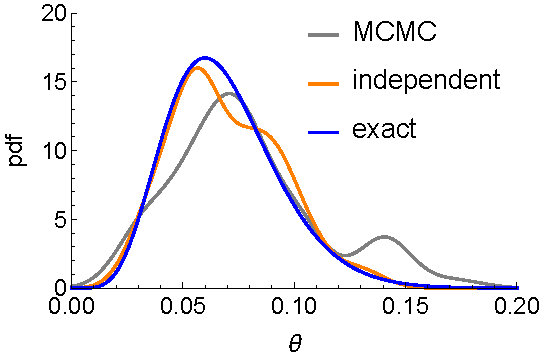
\includegraphics[width=1\textwidth]{../figures/prob3_ticksMCMCIndependentExact.pdf}}
\caption{The estimated posterior via MCMC (orange) and independent (grey) sampling versus the exact posterior (blue).}\label{fig:ticks_independentMCMCIndependentExact}
\end{figure}

\begin{problem}
Run 1000 iterations, where in each iteration you run a single chain for 100 iterations. Store the results in a 1000 x 100 matrix. For each iterate calculate the sample mean. Graph the resultant distribution of sample means. How does MCMC do at estimating the posterior mean?
\end{problem}

With only 100 samples we have not given the chains sufficient time to converge to the posterior density; specifically the effect of using a random start position that is \textit{not} from the posterior means that our posteriors still reflect this. Therefore if we calculate the mean of our 100 posterior samples, it will tend to be upwardly biased of the true value because we haven't allowed for the ``warm-up'' period (figure \ref{fig:ticks_warmup}). 

\begin{problem}
Graph the distribution of the sample mean estimates of the  for the second 50 observations of each chain. How does this result compare with that of the previous question? Why is there a difference?
\end{problem}

The difference is solely due to the warm-up period being discarded (figure \ref{fig:ticks_warmup}). We have allowed the chains time to converge to the posterior, and hence by discarding the first 50 observations we reduce the effect of the random starting position. Since we are now using converged chains the estimator of the mean is unbiased.

\begin{figure}[ht]
\centerline{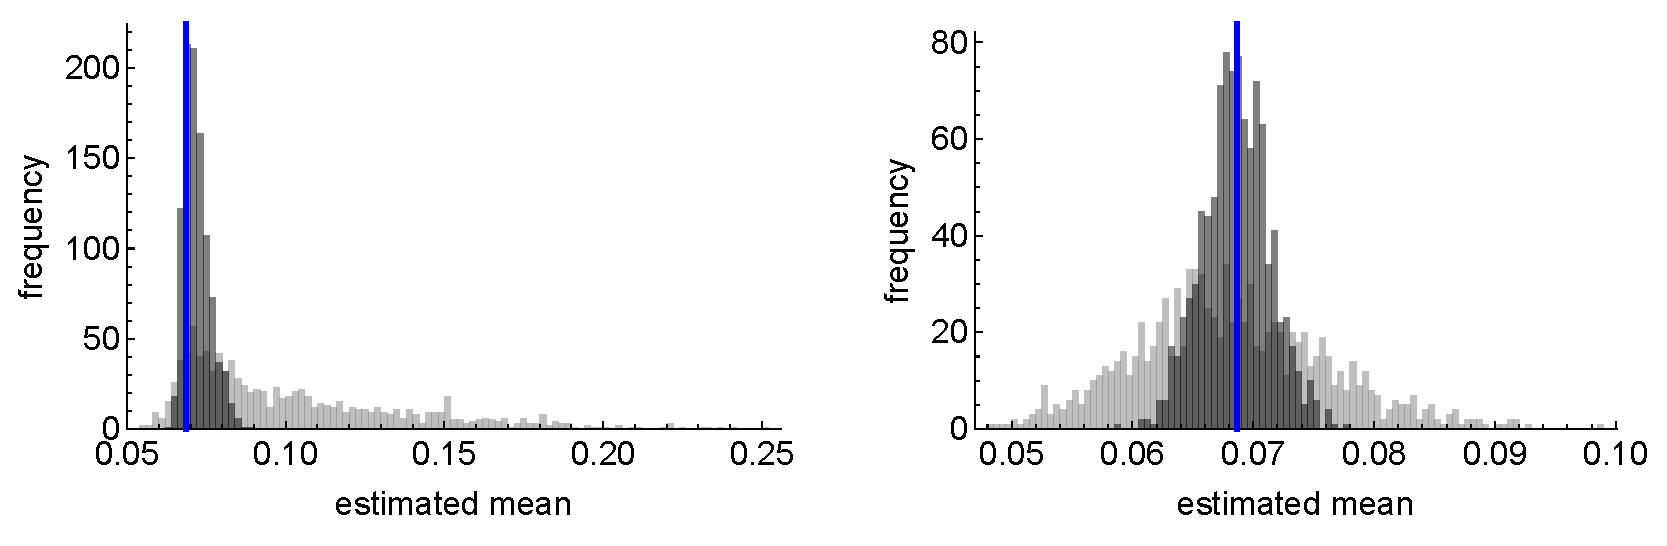
\includegraphics[width=1\textwidth]{../figures/prob3_ticksMCMCMean.pdf}}
\caption{The sampling distribution of the sample mean of the MCMC runs for the ticks example, where (left) we use all 100 samples from each chain, and (right) we only use the second 50.}\label{fig:ticks_warmup}
\end{figure}

\begin{problem}
Decrease the standard deviation (step size) of the proposal distribution to 0.01. For a sample size of 200, how the posterior for a step size of 0.01 compare to that obtained for 0.1?
\end{problem}

A step size of 0.1 is able to find, then explore, the typical set at a much faster rate than the smaller step size (figure \ref{fig:ticks_stepSizeSmall}); meaning that there is a lot of autocorrelation in the sampler's value. Intuitively, a sampler with a small step size is not able to move far from where it was at the end of the previous iteration!

Basically using a step size that is too low is equivalent to using a toothbrush in an archaeological dig. It takes you ages to find any hidden treasures!

\begin{figure}[ht]
\centerline{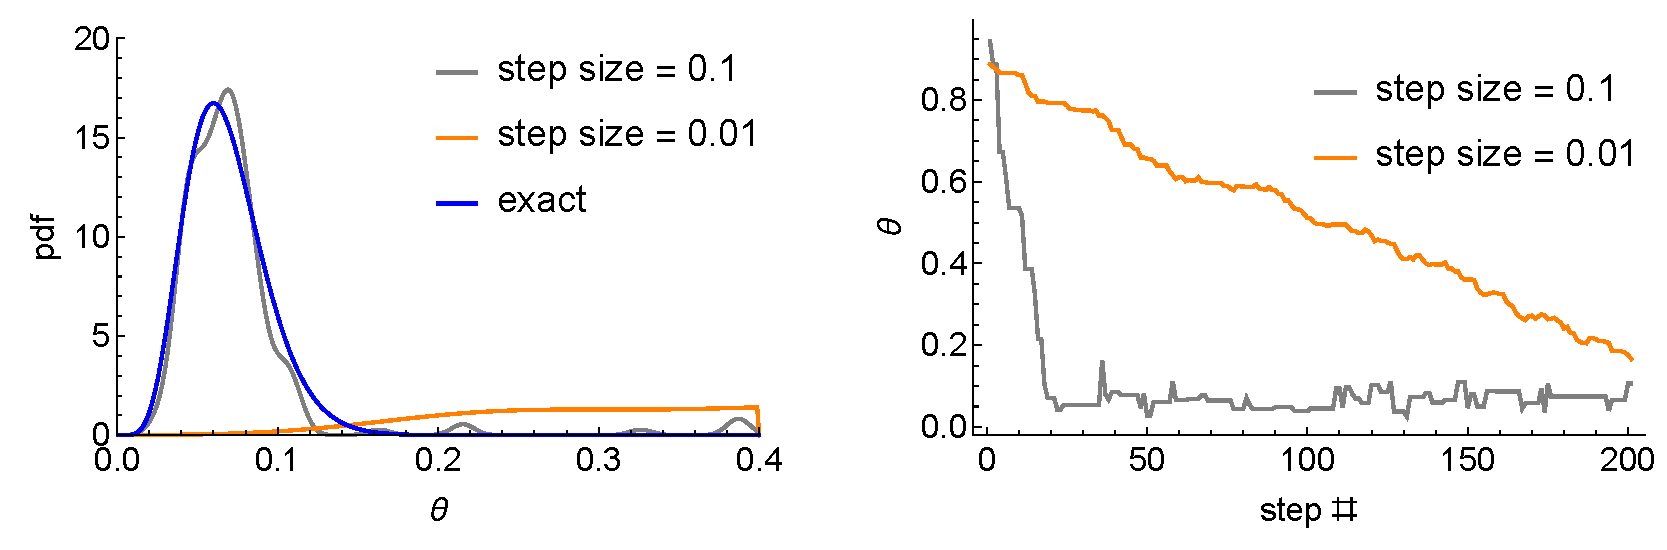
\includegraphics[width=1\textwidth]{../figures/prob3_ticksStepSizeSmall.pdf}}
\caption{Left: the estimated posteriors for two MCMC using two step sizes versus the actual. Right: the evolution of the path of the Markov Chain over time.}\label{fig:ticks_stepSizeSmall}
\end{figure}

\begin{problem}
Increase the standard deviation (step size) of the proposal distribution to 1. For a sample size of 200, how the posterior for a step size of 1 compare to that obtained for 0.1?
\end{problem}

Now the sampler is able to find the typical set fast enough. The trouble now is that it is inefficient at exploring it (figure \ref{fig:ticks_stepSizeLarge}). Intuitively, the path of the sampler is characterised by a high rejection rate, since most of the proposed steps are a long way away from the region of high density.

Overall this means that the reconstructed probability mass at least lies in the correct region of parameter space. However, the reconstructed density has a high variance because there are relatively few unique samples relative to the density from a step size of 0.1.

Basically using a step size that is too large is equivalent to using a digger in an archaeological dig; it finds the treasure fast enough but is too crude to save its finer details.

\begin{figure}[ht]
\centerline{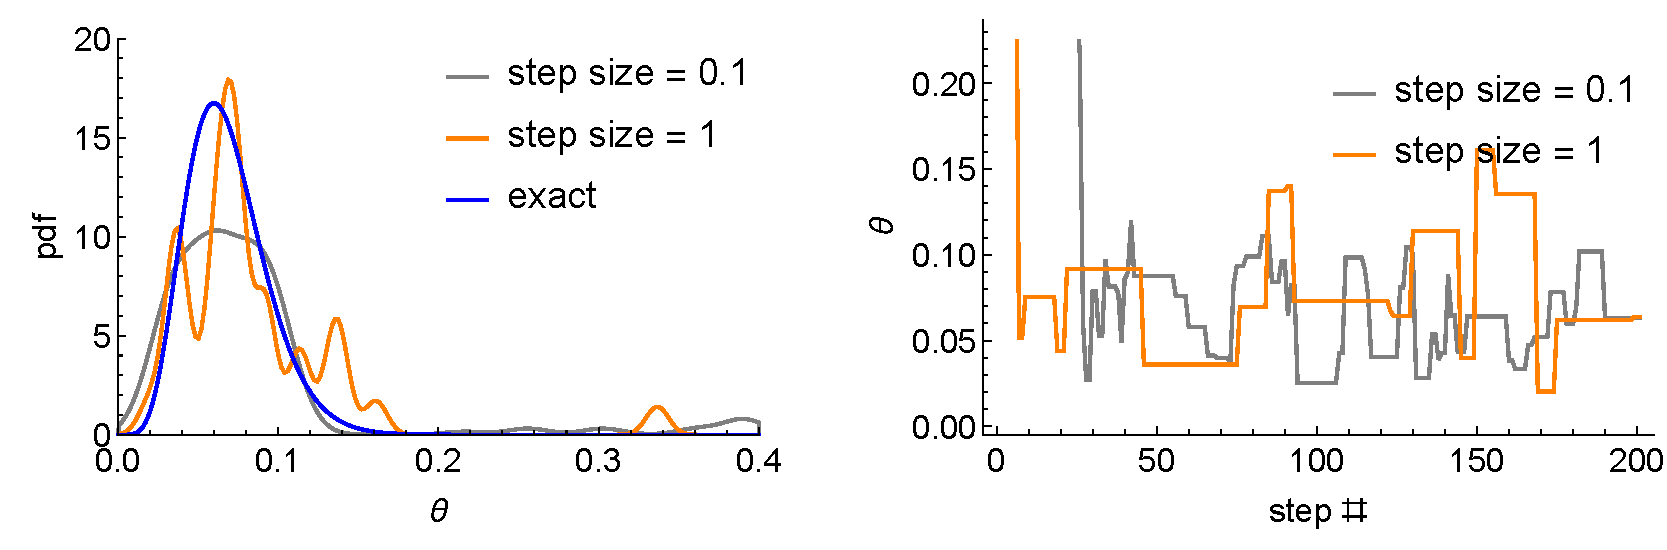
\includegraphics[width=1\textwidth]{../figures/prob3_ticksStepSizeLarge.pdf}}
\caption{Left: the estimated posteriors for two MCMC using two different step sizes versus the actual. Right: the evolution of the path of the Markov Chain over time.}\label{fig:ticks_stepSizeLarge}
\end{figure}


\begin{problem}
Suppose we collect data for a number of such samples (each of size 100), and find the following numbers of ticks that test positive for \textit{Borrelia}: (3,2,8,25). Either calculate the new posterior exactly, or use sampling to estimate it. (Hint: in both cases make sure you include the original sample of 6!)
\end{problem}

The posterior is a Beta(45,457) distribution, which has a mean at about $\theta = 0.09$.

\begin{problem}
Generate samples from the posterior predictive distribution, and use these to test your model. What do these suggest about your model's assumptions?
\end{problem}

Posterior predictive samples are unable to well-replicate either the minimum nor the maximum in the data (figure \ref{fig:ticks_newDataPPCs}). These suggest that either the assumption of independence or identical-distribution is violated; both of which there are good reasons for! (If one tick has the bacteria it will infect nearby animals and in doing so, make it more likely for other ticks to become infected; meaning independence is likely violated. Following on from this we probably think that due to the contagious nature of the disease that there will be hotspots; meaning that the assumption of identical distribution is likely violated.)

\begin{figure}[ht]
\centerline{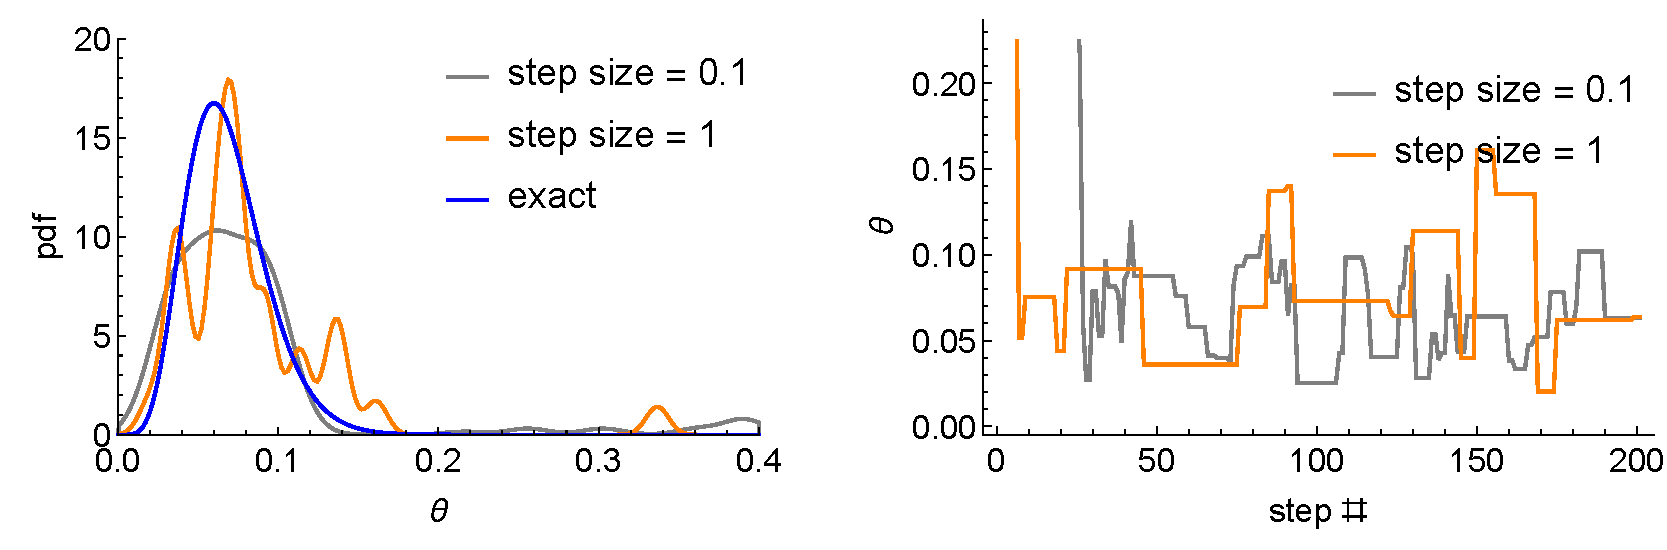
\includegraphics[width=1\textwidth]{../figures/prob3_ticksStepSizeLarge.pdf}}
\caption{The posterior predictive distribution for a dataset of (6,3,2,8,25) \textit{Borrelia}-positive ticks; each out of a sample of 100.}\label{fig:ticks_newDataPPCs}
\end{figure}



\bibliographystyle{plain} 
\bibliography{Bayes}

\end{document}
